\documentclass{article}
\usepackage[utf8]{inputenc}
\usepackage{amsmath}
\usepackage{graphicx}
\usepackage{geometry}
\usepackage{tikz} % Dodan paket za crtanje
\usetikzlibrary{arrows.meta, calc} % Dodane potrebne TikZ biblioteke

\geometry{a4paper, margin=1in}

\title{Matematički Izvod Dinamike Sustava Kolica s Njihalom}
\author{Euler-Lagrangeova Metoda}
\date{\today}

\begin{document}

\maketitle

\section{Uvod}
Ovaj dokument detaljno opisuje izvod nelinearnih jednadžbi dinamike za sustav kolica s njihalom (eng. cart-pendulum) korištenjem Euler-Lagrangeove metode. Sustav se sastoji od kolica mase \(M\) koja se mogu gibati horizontalno i njihala mase \(m\) i duljine \(L\) koje je zglobno povezano s kolicima.

\begin{figure}[h!]
    \centering
    % TikZ kod za crtanje sheme sustava
    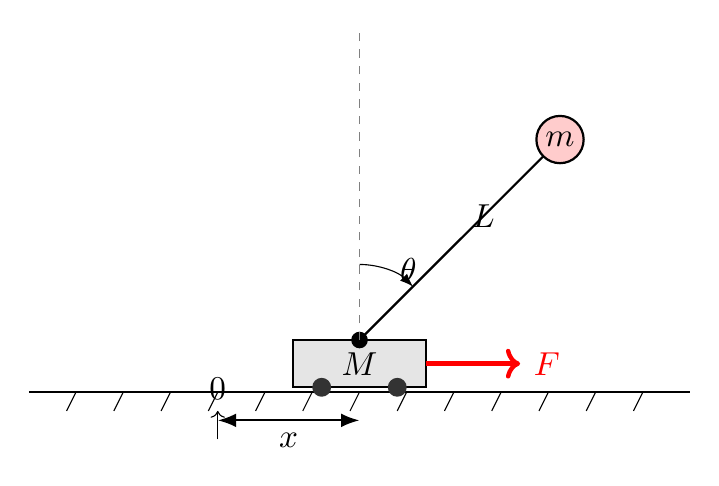
\begin{tikzpicture}[scale=1.2, every node/.style={scale=1.2}]
        % Definicija varijabli za lakše pozicioniranje
        \def\cartX{1.5} % x-pozicija kolica
        \def\pendulumAngle{45} % Kut njihala od vertikale (prema dolje)
        \def\pendulumLength{3} % Duljina njihala

        % Podloga
        \draw[thick] (-2,0) -- (5,0);
        \foreach \x in {-1.5, -1, ..., 4.5} {
            \draw (\x, 0) -- (\x-0.1, -0.2);
        }

        % Kolica (Cart)
        \draw[thick, fill=gray!20] (\cartX-0.7, 0.05) rectangle (\cartX+0.7, 0.55);
        \node at (\cartX, 0.3) {\(M\)};
        \fill[black!80] (\cartX-0.4, 0.05) circle (0.1);
        \fill[black!80] (\cartX+0.4, 0.05) circle (0.1);

        % Koordinatni sustav i pozicija x
        \draw[->, thin] (0, -0.5) -- (0, -0.2) node[above] {$0$};
        \draw[<->, >=Latex, thick] (0, -0.3) -- (\cartX, -0.3) node[midway, below] {$x$};
        
        % Njihalo (Pendulum)
        % Pivot točka
        \coordinate (pivot) at (\cartX, 0.55);
        % Pozicija mase njihala (koristi se 'calc' biblioteka)
        \coordinate (mass) at ($(pivot) + (90-\pendulumAngle:\pendulumLength)$);
        
        % Šipka njihala
        \draw[thick] (pivot) -- (mass) node[midway, above right] {\(L\)};
        % Zglob (pivot point) nacrtan kao puni krug
        \fill[black] (pivot) circle (2.5pt);

        % Masa njihala
        \draw[thick, fill=red!20] (mass) circle (0.25cm);
        \node at (mass) {\(m\)};

        % Vertikalna isprekidana linija za kut
        \draw[dashed, gray] (pivot) -- ++(0, \pendulumLength*1.1);

        % Oznaka za kut theta (koristi se 'calc' biblioteka)
        \draw[->, >=Latex] ($(pivot) + (90:0.8)$) arc (90:90-\pendulumAngle:0.8) node[midway, right] {$\theta$};

        % Sila F
        \draw[->, ultra thick, red] (\cartX+0.7, 0.3) -- ++(1,0) node[right] {$F$};

    \end{tikzpicture}
    \caption{Shematski prikaz sustava kolica s njihalom, generiran pomoću TikZ.}
    \label{fig:shema}
\end{figure}

\section{Definiranje Koordinata}
Generalizirane koordinate koje opisuju položaj sustava su:
\begin{itemize}
    \item \(x\): horizontalni položaj kolica.
    \item \(\theta\): kut njihala u odnosu na vertikalu (mjereno od donjeg stabilnog položaja, \(\theta = \pi\) je gornji nestabilni položaj).
\end{itemize}

Položaj centra mase njihala (\(x_p, y_p\)) može se izraziti kao:
\begin{align}
    x_p &= x + L \sin(\theta) \\
    y_p &= L \cos(\theta)
\end{align}

Brzine centra mase njihala dobivamo deriviranjem po vremenu:
\begin{align}
    \dot{x}_p &= \dot{x} + L \cos(\theta) \dot{\theta} \\
    \dot{y}_p &= -L \sin(\theta) \dot{\theta}
\end{align}

\section{Energije Sustava}

\subsection{Kinetička Energija (T)}
Ukupna kinetička energija sustava zbroj je kinetičke energije kolica \(T_c\) i kinetičke energije njihala \(T_p\).

Kinetička energija kolica:
\begin{equation}
    T_c = \frac{1}{2} M \dot{x}^2
\end{equation}

Kinetička energija njihala (pretpostavljamo da je masa koncentrirana na kraju štapa):
\begin{equation}
    T_p = \frac{1}{2} m (\dot{x}_p^2 + \dot{y}_p^2)
\end{equation}
\begin{align*}
    T_p &= \frac{1}{2} m ((\dot{x} + L \cos(\theta) \dot{\theta})^2 + (-L \sin(\theta) \dot{\theta})^2) \\
    &= \frac{1}{2} m (\dot{x}^2 + 2 \dot{x} L \cos(\theta) \dot{\theta} + L^2 \cos^2(\theta) \dot{\theta}^2 + L^2 \sin^2(\theta) \dot{\theta}^2) \\
    &= \frac{1}{2} m (\dot{x}^2 + 2 \dot{x} L \cos(\theta) \dot{\theta} + L^2 \dot{\theta}^2)
\end{align*}

Ukupna kinetička energija sustava je \(T = T_c + T_p\):
\begin{equation}
    T = \frac{1}{2} (M+m)\dot{x}^2 + m L \cos(\theta) \dot{x} \dot{\theta} + \frac{1}{2} m L^2 \dot{\theta}^2
\end{equation}

\subsection{Potencijalna Energija (V)}
Potencijalna energija ovisi samo o visini njihala. Postavljamo referentnu nultu razinu na visinu zgloba (\(y=0\)).
\begin{equation}
    V = m g y_p = m g L \cos(\theta)
\end{equation}

\section{Lagrangeova Funkcija}
Lagrangeova funkcija \(L\) definirana je kao \(L = T - V\).
\begin{equation}
    \mathcal{L} = \frac{1}{2} (M+m)\dot{x}^2 + m L \cos(\theta) \dot{x} \dot{\theta} + \frac{1}{2} m L^2 \dot{\theta}^2 - m g L \cos(\theta)
\end{equation}

\section{Euler-Lagrangeove Jednadžbe}
Jednadžbe gibanja dobivamo iz Euler-Lagrangeovih jednadžbi za svaku generaliziranu koordinatu:
\begin{equation}
    \frac{d}{dt}\left(\frac{\partial \mathcal{L}}{\partial \dot{q}_i}\right) - \frac{\partial \mathcal{L}}{\partial q_i} = Q_i
\end{equation}
gdje je \(q_i\) generalizirana koordinata, a \(Q_i\) generalizirana sila koja djeluje na tu koordinatu.

\subsection{Jednadžba za koordinatu \(x\)}
Za koordinatu \(x\), generalizirana sila je vanjska sila \(F\) koja djeluje na kolica, dakle \(Q_x = F\).

Prvo računamo parcijalne derivacije:
\begin{align*}
    \frac{\partial \mathcal{L}}{\partial x} &= 0 \\
    \frac{\partial \mathcal{L}}{\partial \dot{x}} &= (M+m)\dot{x} + m L \cos(\theta) \dot{\theta}
\end{align*}
Sada deriviramo po vremenu:
\begin{equation*}
    \frac{d}{dt}\left(\frac{\partial \mathcal{L}}{\partial \dot{x}}\right) = (M+m)\ddot{x} + m L \cos(\theta) \ddot{\theta} - m L \sin(\theta) \dot{\theta}^2
\end{equation*}
Uvrštavanjem u Euler-Lagrangeovu jednadžbu dobivamo prvu jednadžbu gibanja:
\begin{equation}
    (M+m)\ddot{x} + m L \cos(\theta) \ddot{\theta} - m L \sin(\theta) \dot{\theta}^2 = F
\end{equation}

\subsection{Jednadžba za koordinatu \(\theta\)}
Za koordinatu \(\theta\), nema vanjskog momenta koji djeluje na njihalo, pa je \(Q_\theta = 0\).

Računamo parcijalne derivacije:
\begin{align*}
    \frac{\partial \mathcal{L}}{\partial \theta} &= -m L \sin(\theta) \dot{x} \dot{\theta} + m g L \sin(\theta) \\
    \frac{\partial \mathcal{L}}{\partial \dot{\theta}} &= m L \cos(\theta) \dot{x} + m L^2 \dot{\theta}
\end{align*}
Deriviramo po vremenu:
\begin{equation*}
    \frac{d}{dt}\left(\frac{\partial \mathcal{L}}{\partial \dot{\theta}}\right) = m L \cos(\theta) \ddot{x} - m L \sin(\theta) \dot{\theta} \dot{x} + m L^2 \ddot{\theta}
\end{equation*}
Sada uvrštavamo u Euler-Lagrangeovu jednadžbu:
\begin{align*}
    (m L \cos(\theta) \ddot{x} - m L \sin(\theta) \dot{\theta} \dot{x} + m L^2 \ddot{\theta}) - (-m L \sin(\theta) \dot{x} \dot{\theta} + m g L \sin(\theta)) = 0 \\
    m L \cos(\theta) \ddot{x} + m L^2 \ddot{\theta} - m g L \sin(\theta) = 0
\end{align*}
Dijeljenjem s \(mL\) dobivamo drugu jednadžbu gibanja:
\begin{equation}
    L \cos(\theta) \ddot{x} + L^2 \ddot{\theta} - g L \sin(\theta) = 0 \implies \ddot{x} \cos(\theta) + L \ddot{\theta} - g \sin(\theta) = 0
\end{equation}

\section{Zaključak: Nelinearne Jednadžbe Gibanja}
Sustav nelinearnih diferencijalnih jednadžbi koje opisuju dinamiku sustava kolica s njihalom su:
\begin{align}
    (M+m)\ddot{x} + m L \cos(\theta) \ddot{\theta} - m L \sin(\theta) \dot{\theta}^2 &= F \\
    \ddot{x} \cos(\theta) + L \ddot{\theta} - g \sin(\theta) &= 0
\end{align}
Ove dvije jednadžbe čine nelinearni model sustava. Za potrebe simulacije i upravljanja, potrebno ih je riješiti po \(\ddot{x}\) i \(\ddot{\theta}\).

\end{document}

